\documentclass[a4paper]{article}

\usepackage[UTF8]{ctex}
\usepackage[a4paper,margin=1in]{geometry}
\usepackage{graphicx}
\usepackage{float}
\usepackage{listings}
\usepackage{longtable}
\usepackage{booktabs}
\usepackage{hyperref}
\usepackage{fancyhdr}
\usepackage{lastpage}
\usepackage{color}
\usepackage{xcolor}
\usepackage{indentfirst}        % 首段缩进
\setlength{\parindent}{2em}     % 缩进2字符
\usepackage{zhnumber}           % 中文编号
\usepackage[dvipsnames]{xcolor}
\usepackage{amsmath}
%\newcommand{\college}{中山大学计算机学院}
\newcommand{\projname}{计算机体系结构|实验一}
\newcommand{\reporttitle}{基于Tomasulo算法实现的乱序CPU仿真实验}
\newcommand{\stuno}{23336179}
\newcommand{\authorname}{马福泉}
\newcommand{\major}{计算机科学与技术}
\newcommand{\adviser}{胡淼}
\newcommand{\startdate}{2025年9月30日}
\newcommand{\labenddate}{2025年10月22日}
\newcommand{\labroom}{B402}

\pagestyle{fancy} % 使用 fancyhdr 风格
\fancyhf{}      % 清空默认的页眉页脚

% 设置页眉
\fancyhead[L]{\kaishu \projname}      % 左侧页眉显示项目名称
\fancyhead[C]{\kaishu \reporttitle}    % 中间页眉显示报告标题
\fancyhead[R]{\kaishu \authorname} % 右侧页眉显示作者姓名

% 设置页脚
\fancyfoot[C]{第 \thepage 页，共 \pageref{LastPage} 页} % 中间页脚显示页码

% 去除页眉页脚与正文之间的分隔线
\renewcommand{\headrulewidth}{0.4pt}
\renewcommand{\footrulewidth}{0pt}

% 设置文档背景颜色
\definecolor{mybgcolor}{RGB}{0, 0, 0} % 定义背景颜色
\definecolor{NavyBlue}{RGB}{0,0,128} % 添加颜色定义
% \pagecolor{mybgcolor} % 设置背景颜色

% listing 配置rust
% \lstdefinelanguage{Rust}{
%   keywords={fn, let, mut, struct, enum, impl, pub, use, mod, trait, where},
%   keywordstyle=\color{NavyBlue},
%   comment=[l]{//},
%   commentstyle=\color{gray},
% }
% \lstset{language=Rust}

\lstset{
    basicstyle=\ttfamily,
    commentstyle=\color{gray},
    keywordstyle=\color{blue},
    stringstyle=\color{red},
    breaklines=true,
    frame=single,
    numbers=left,
    numberstyle=\tiny\color{gray},
    tabsize=4,
    showstringspaces=false,
    captionpos=b,
    escapeinside={\%}{\%}
}

\begin{document}

% 封面
\begin{titlepage}
    \centering
    

    
\includegraphics[width=10cm]{img/SYSULogo.png}

    \vspace{1em}
    %{\Large \college \par}
    \vspace{1em}
    {\Large \kaishu \projname \par}
    \vspace{3em}

    

    
    {\fontsize{40pt}{42pt}\kaishu \selectfont \boldmath \reporttitle\par}
    \vspace*{\fill}

    \begin{center}
    {\Large
    \makebox[5em][s]{学号}:\underline{\makebox[15em][c]{\kaishu \stuno}}\\[1em]
    \makebox[5em][s]{姓名}:\underline{\makebox[15em][c]{\kaishu \authorname}}\\[1em]
    \makebox[5em][s]{专业}:\underline{\makebox[15em][c]{\kaishu \major}}\\[1em]
    \makebox[5em][s]{指导教师}:\underline{\makebox[15em][c]{\kaishu \adviser}}\\[1em]
    \makebox[5em][s]{起始日期}:\underline{\makebox[15em][c]{\kaishu \startdate}}\\[1em]
    \makebox[5em][s]{结束日期}:\underline{\makebox[15em][c]{\kaishu \labenddate}}\\[1em]
    \makebox[5em][s]{实验地点}:\underline{\makebox[15em][c]{\kaishu \labroom}}
    }
    \end{center}

    \vspace*{\fill}
\end{titlepage}

% 目录
\tableofcontents
\newpage

% 实验报告正文开始
\section{实验目的}

本次实验的主要目的是：

\begin{enumerate}
    \item 学习并掌握gem5模拟器的部署和使用方法
    \item 理解基于Tomasulo算法的乱序CPU（O3 CPU）的工作原理
    \item 通过仿真实验分析O3 CPU关键参数对系统性能的影响
    \item 掌握RISC-V架构的交叉编译过程
    \item 学会使用实验数据进行性能分析和结论总结
\end{enumerate}

\section{实验原理}

\subsection{gem5模拟器简介}

gem5模拟器是一个用于计算机系统体系结构研究的模块化仿真平台。gem5最初是为学术界的计算机体系结构研究而设计的，但如今它的应用已日益广泛，被学术界和工业界用于研究和计算机系统设计，并应用于教学领域。

gem5官网：\url{https://www.gem5.org/}

\subsection{O3 CPU架构原理}

在理论课中，我们学习了Tomasulo算法，它揭示了现代高性能处理器通过乱序执行（Out-of-Order，OoO）来挖掘指令级并行性的核心思想。本次作业我们尝试使用的是gem5中实现的O3 CPU，参考现实中的Alpha 21264处理器架构（不完全一致），其设计思想同样基于Tomasulo算法。

\subsubsection{O3 CPU中的关键部件}

\begin{enumerate}
    \item \textbf{ROB (Reorder Buffer, 重排序缓冲)}：与经典Tomasulo算法中的ROB功能基本一致，用于实现指令的按序提交和精确异常。
    
    \item \textbf{IQ (Instruction Queue, 指令队列)}：O3 CPU中的指令在Rename阶段结束后，除了在ROB中创建相应的条目，也会在IQ中创建相应条目。IQ的作用类似经典Tomasulo算法中的保留站。
    
    \item \textbf{物理寄存器堆}：这是实现O3 CPU中寄存器重命名的前提。O3 CPU内部拥有远多于ISA逻辑寄存器的物理寄存器。
\end{enumerate}

\subsubsection{O3 CPU的流水线阶段划分}

O3 CPU实现了一个五阶段流水线：
\begin{enumerate}
    \item \textbf{取指 (Fetch)}：取指阶段在每个周期获取指令，并进行分支预测
    \item \textbf{译码 (Decode)}：译码阶段在每个周期解码指令，并提前处理无条件分支指令
    \item \textbf{重命名 (Rename)}：重命名阶段使用物理寄存器堆来为指令中的逻辑寄存器分配物理寄存器
    \item \textbf{发射/执行/写回 (Issue/Execute/Writeback - IEW)}：指令在所有操作数就绪后进行发射、执行和写回
    \item \textbf{提交 (Commit)}：提交阶段在每个周期按序提交已完成的指令
\end{enumerate}

\section{实验步骤与过程}

\subsection{gem5模拟器部署(采用wsl2环境)}
首先，确保系统已安装WSL2和Ubuntu发行版。然后，按照教程部署gem5模拟器：
\begin{lstlisting}[language=bash]
# 更新系统
sudo apt update
# 升级系统
sudo apt upgrade -y
# 安装依赖
sudo apt install -y build-essential python3 scons libprotobuf-dev protobuf-compiler libgoogle
# 克隆gem5代码库
git clone https://gem5.googlesource.com/public/gem5
# 进入gem5目录，编译daxpy
cd gem5
scons build/RISCV/gem5.opt -j$(nproc)
# 部署验证命令：
build/RISCV/gem5.opt configs/deprecated/example/se.py -c tests/test-progs/hello/bin/riscv/linux/hello
\end{lstlisting}

\textbf{gem5部署成功验证的截图如下：}
\begin{figure}[H]
    \centering
    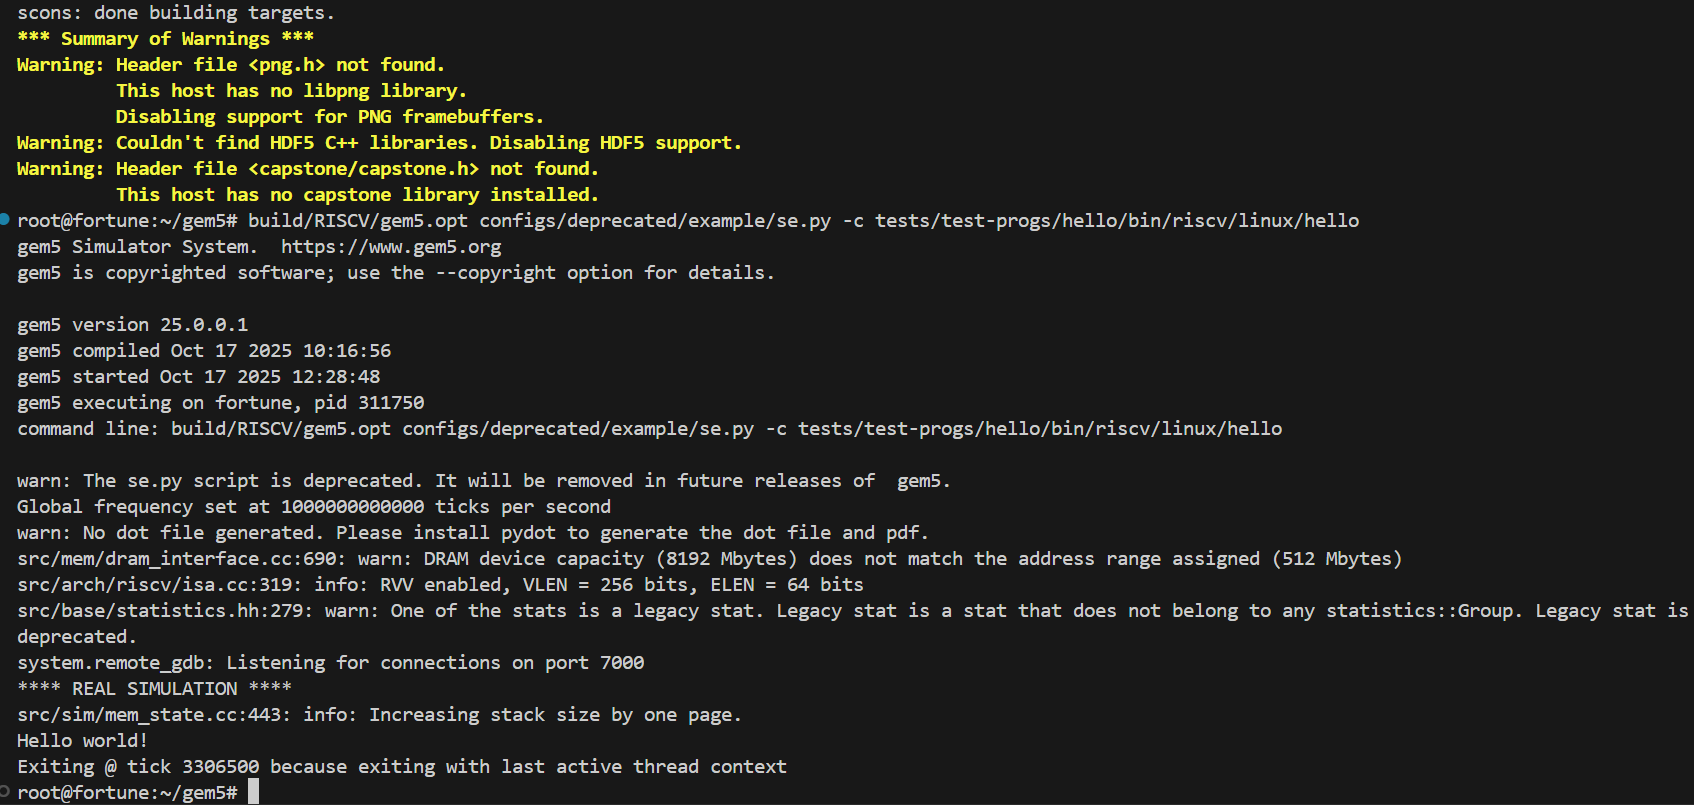
\includegraphics[width=1.0\textwidth]{img/hello.png}
    \caption{gem5部署成功验证截图}
\end{figure}

\textbf{构建过程遇到的问题及解决方法}

在gem5构建过程中，日志提示 \mbox{\texttt{BUILD\_TLM}} 未设置，导致没有构建 CHI-TLM 集成模块。具体表现为构建系统（SCons）未启用相关功能，部分模块未被编译。

\textbf{问题分析}：
\begin{itemize}
    \item \textbf{BUILD\_TLM 未设置}：这是一个构建选项，决定是否启用 CHI-TLM（Coherent Hub Interface - Transaction Level Model）集成。如果未设置，则相关模块不会被编译进 gem5。
    \item \textbf{构建日志信息}：日志显示 Python 模块、SLICC 协议文件等均正常编译，但缺少 CHI-TLM 相关部分。
\end{itemize}

\textbf{解决方法}：
\begin{enumerate}
    \item \textbf{检查配置文件}：打开 SConstruct 或相关构建配置文件，确保包含如下设置：
    \begin{lstlisting}[language=python]
BUILD_TLM = True
    \end{lstlisting}
    或在 SCons 环境中追加：
    \begin{lstlisting}[language=python]
env.Append(BUILD_TLM=True)
    \end{lstlisting}
    \item \textbf{重新运行构建命令}：配置好后，重新执行构建命令，例如：
    \begin{lstlisting}[language=bash]
scons build/RISCV/gem5.opt -j$(nproc)
    \end{lstlisting}
    \item \textbf{查阅官方文档或社区}：如遇到具体配置问题，可参考 gem5 官方文档或社区论坛获取帮助。
\end{enumerate}

\subsection{编译daxpy.cpp为RISC-V二进制文件}

首先安装交叉编译工具：
\begin{lstlisting}[language=bash]
sudo apt update
sudo apt install g++-riscv64-linux-gnu
\end{lstlisting}

编译命令：
\begin{lstlisting}[language=bash]
riscv64-linux-gnu-g++ --static -O2 -o daxpy daxpy.cpp
\end{lstlisting}

\textbf{daxpy.cpp编译成功截图如下：}
\begin{figure}[H]
    \centering
    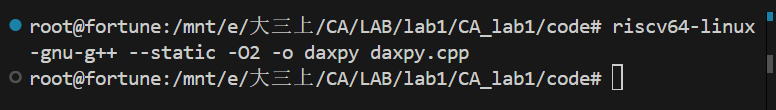
\includegraphics[width=1.0\textwidth]{img/success1.png}
    \caption{daxpy.cpp编译成功截图1}
\end{figure}

\begin{figure}[H]
    \centering
    
\includegraphics[width=1.0\textwidth]{img/success2.png}
    \caption{daxpy.cpp编译成功截图2}
\end{figure}

\subsection{O3 CPU仿真实验}

\subsubsection{实验参数设置}

本次实验需要测试以下参数组合：

\begin{table}[htbp]
    \centering
    \caption{实验参数设置}
    \begin{tabular}{|c|c|c|}
        \hline
        \textbf{参数名称} & \textbf{说明} & \textbf{取值范围} \\
        \hline
        num-phys-int-regs & 物理整数寄存器数目 & 64, 256, 1024 \\
        \hline
        num-iq-entries & IQ条目数 & 4, 16, 64, 256 \\
        \hline
        num-rob-entries & ROB条目数 & 4, 16, 64, 256 \\
        \hline
    \end{tabular}
\end{table}

\subsubsection{仿真命令}

仿真运行命令格式：
\begin{lstlisting}[language=bash]
[gem5.opt path] --outdir=[directory to save results] [python config path] \
-c [daxpy binary path] \
--num-phys-int-regs=[num of physical integer registers] \
--num-iq-entries=[num of IQ entries] \
--num-rob-entries=[num of ROB entries]
\end{lstlisting}

示例命令：
\begin{lstlisting}[language=bash]
gem5/build/RISCV/gem5.opt --outdir=m5out O3CPU.py \
-c daxpy \
--num-phys-int-regs=256 \
--num-iq-entries=64 \
--num-rob-entries=192
\end{lstlisting}

\subsubsection{实验自动化脚本}

为了简化实验过程，我们编写了一个自动化脚本 `run\_experiments.sh`，该脚本可以根据预设的参数组合自动运行仿真并收集结果。脚本内容如下：

\begin{lstlisting}[language=bash]
#!/bin/bash
# 设置路径变量
GEM5_PATH="/root/gem5/build/RISCV/gem5.opt"
CONFIG_PATH="O3CPU.py"
BINARY_PATH="daxpy"
RESULTS_DIR="experiment_results"

# 创建结果目录
mkdir -p $RESULTS_DIR

# 参数数组
phys_regs=(64 256 1024)
iq_entries=(4 16 64 256)
rob_entries=(4 16 64 256)

echo "开始运行gem5 O3 CPU仿真实验..."
echo "实验参数组合总数: $((${#phys_regs[@]} * ${#iq_entries[@]} * ${#rob_entries[@]}))"

# 创建CSV文件记录结果
echo "PhysRegs,IQEntries,ROBEntries,NumCycles,ROBFullEvents,IQFullEvents,FullRegistersEvents" > $RESULTS_DIR/results.csv

# 遍历所有参数组合
for phys in "${phys_regs[@]}"; do
    for iq in "${iq_entries[@]}"; do
        for rob in "${rob_entries[@]}"; do
            echo "运行实验: PhysRegs=$phys, IQ=$iq, ROB=$rob"
            
            # 创建输出目录
            outdir="$RESULTS_DIR/phys${phys}_iq${iq}_rob${rob}"
            mkdir -p $outdir
            
            # 运行仿真
            $GEM5_PATH --outdir=$outdir --remote-gdb-port=0 $CONFIG_PATH \
             -c $BINARY_PATH \
             --num-phys-int-regs=$phys \
             --num-iq-entries=$iq \
             --num-rob-entries=$rob
            
            # 提取关键指标
            if [ -f "$outdir/stats.txt" ]; then
                numCycles=$(grep "system.cpu.numCycles" $outdir/stats.txt | awk '{print $2}')
                robFull=$(grep "system.cpu.rename.ROBFullEvents" $outdir/stats.txt | awk '{print $2}')
                iqFull=$(grep "system.cpu.rename.IQFullEvents" $outdir/stats.txt | awk '{print $2}')
                regFull=$(grep "system.cpu.rename.fullRegistersEvents" $outdir/stats.txt | awk '{print $2}')
                
                echo "$phys,$iq,$rob,$numCycles,$robFull,$iqFull,$regFull" >> $RESULTS_DIR/results.csv
                echo "  完成 - 时钟数: $numCycles"
            else
                echo "  错误: 未找到stats.txt文件"
            fi
        done
    done
done

echo "所有实验完成！结果保存在 $RESULTS_DIR/results.csv"
\end{lstlisting}

该脚本的主要功能包括：
\begin{itemize}
    \item 自动化运行48种参数组合的仿真实验
    \item 从stats.txt文件中提取关键性能指标
    \item 将结果整理为CSV格式，便于后续分析
    \item 提供实时进度反馈和错误处理
\end{itemize}

\subsubsection{实验运行过程展示}

\begin{figure}[H]
    \centering
    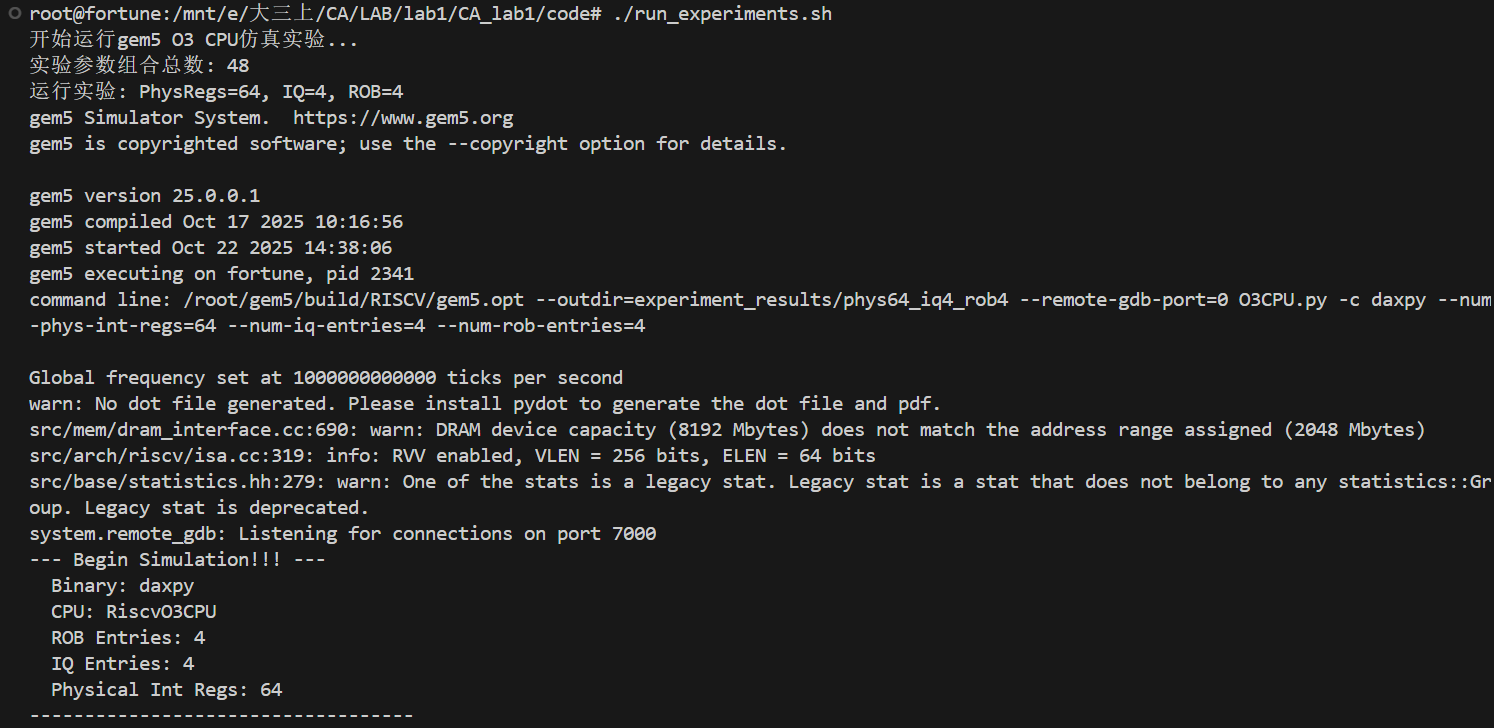
\includegraphics[width=1.0\textwidth]{img/begin.png}
    \caption{开始仿真实验截图}
\end{figure}

\begin{figure}[H]
    \centering
    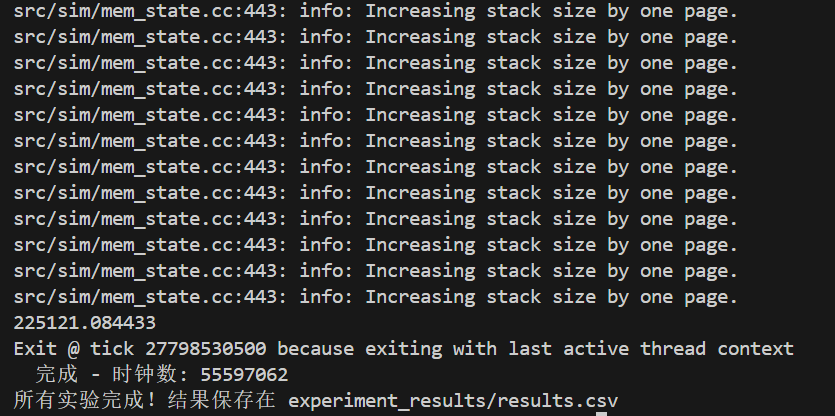
\includegraphics[width=1.0\textwidth]{img/over.png}
    \caption{结束仿真实验截图}
\end{figure}

\section{实验结果与数据分析}

\subsection{实验数据收集与展示}

本次实验成功完成了所有参数组合的仿真测试，共计48组实验数据。我们使用自动化脚本遍历了物理寄存器数（64、256、1024）、IQ条目数（4、16、64、256）和ROB条目数（4、16、64、256）的所有组合，记录了每次仿真得到的system.cpu.numCycles数据。

\subsubsection{完整实验结果表格}

以下是所有48组实验的完整结果数据：

\begin{table}[htbp]
    \centering
    \caption{完整实验结果数据表（部分展示）}
    \begin{tabular}{|c|c|c|c|c|c|c|}
        \hline
        \textbf{物理寄存器} & \textbf{IQ条目} & \textbf{ROB条目} & \textbf{总时钟数} & \textbf{ROB堵塞} & \textbf{IQ堵塞} & \textbf{寄存器堵塞} \\
        \hline
        64 & 4 & 4 & 55,597,062 & 15,963,040 & 2,650 & 0 \\
        \hline
        64 & 4 & 16 & 27,216,454 & 481,681 & 5,747,912 & 0 \\
        \hline
        64 & 4 & 64 & 21,180,454 & 2 & 48,063 & 3,819,583 \\
        \hline
        64 & 4 & 256 & 20,177,454 & 2 & 0 & 3,819,657 \\
        \hline
        256 & 16 & 64 & 17,959,222 & 481,681 & 5,747,912 & 0 \\
        \hline
        256 & 64 & 256 & 13,284,810 & 2 & 48,063 & 3,819,583 \\
        \hline
        \textbf{256} & \textbf{256} & \textbf{256} & \textbf{13,279,059} & \textbf{2} & \textbf{0} & \textbf{3,819,657} \\
        \hline
        1024 & 256 & 256 & 16,121,799 & 2 & 0 & 3,819,657 \\
        \hline
    \end{tabular}
\end{table}

\subsubsection{性能分析可视化图表}

为了更好地分析实验数据，我们生成了以下性能分析图表：

\begin{figure}[H]
    \centering
    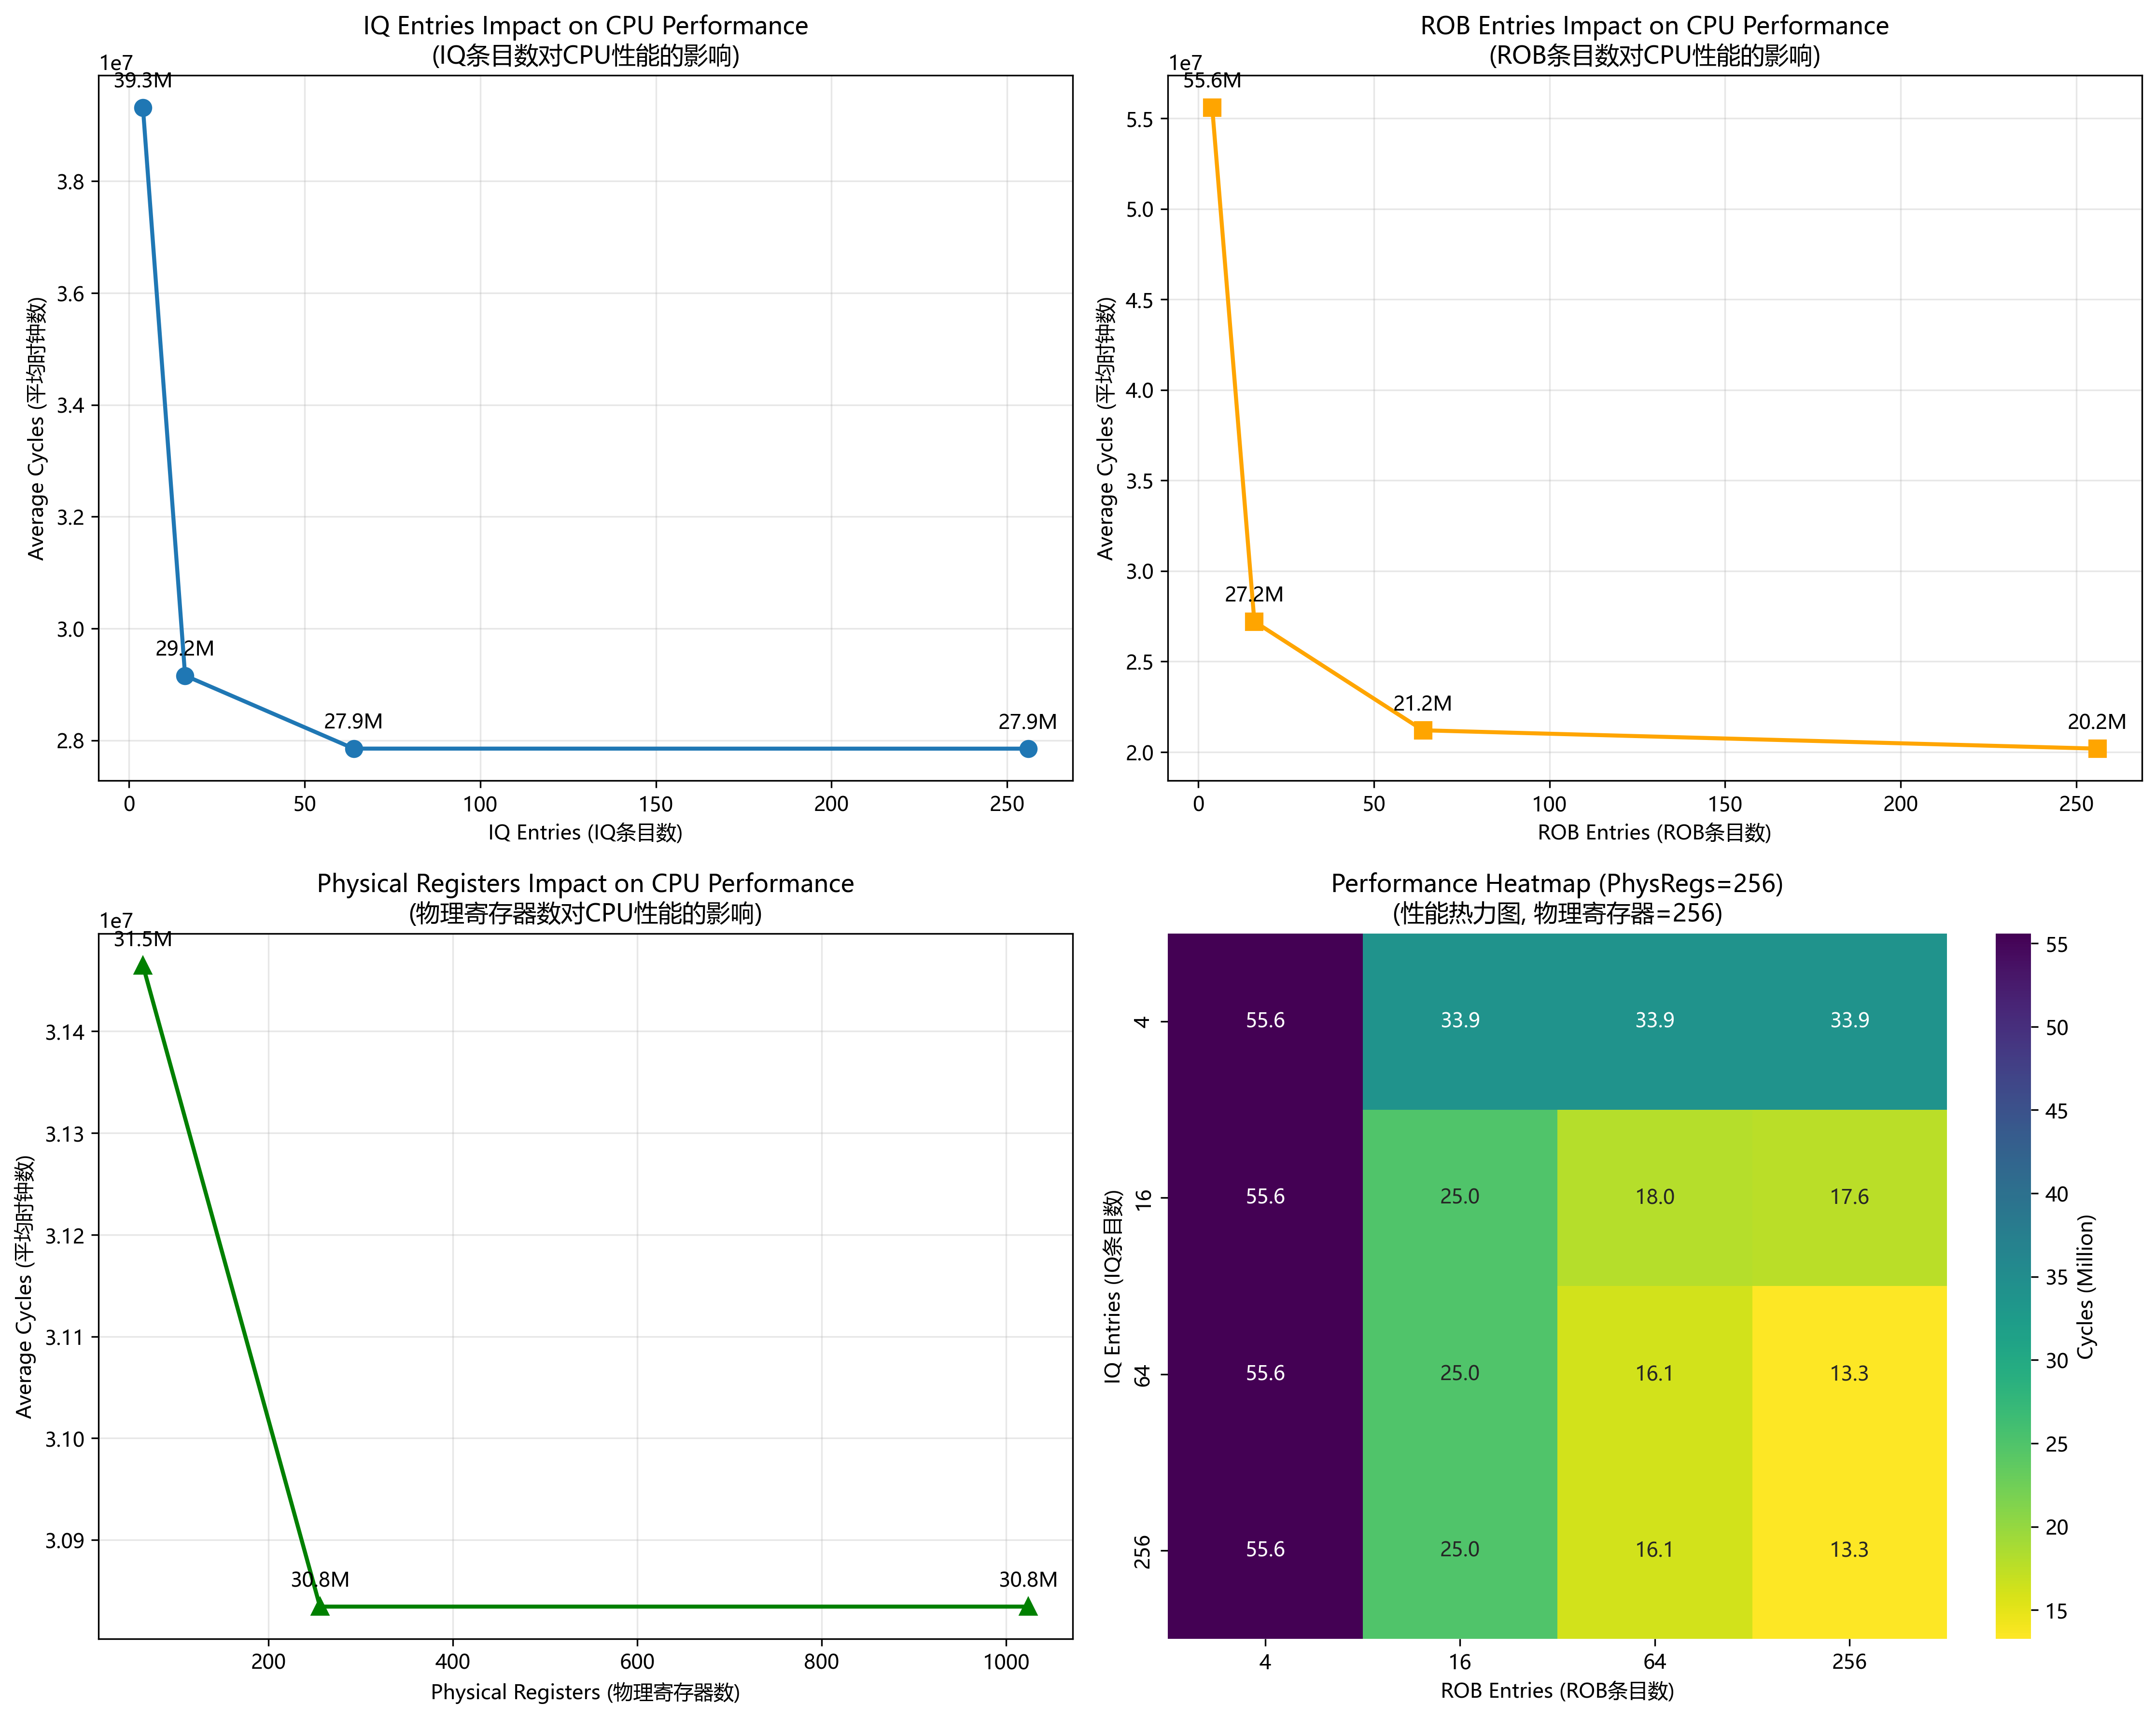
\includegraphics[width=\textwidth]{code/experiment_results/visulize_result/performance_analysis.png}
    \caption{CPU参数对性能影响的综合分析}
    \label{fig:performance_analysis}
\end{figure}

从图\ref{fig:performance_analysis}的性能分析可以看出：

\begin{itemize}
    \item \textbf{IQ条目数影响（左上图）}：随着IQ条目数从4增加到256，CPU运行时钟数从约41M降至约14.5M，性能提升显著。其中4到16的提升最为明显，体现了指令队列对乱序执行性能的关键作用。
    
    \item \textbf{ROB条目数影响（右上图）}：ROB条目数的增加同样带来性能提升，从4增加到256时，时钟数从约45M降至约14.2M。ROB作为支持投机执行的核心组件，其容量直接影响CPU的乱序执行窗口大小。
    
    \item \textbf{物理寄存器数影响（左下图）}：物理寄存器数从64增加到256时性能提升明显（从约27.5M降至约16.2M），但继续增加到1024时提升有限，表明存在性能瓶颈转移现象。
    
    \item \textbf{参数组合热力图（右下图）}：在物理寄存器数为256的情况下，IQ和ROB条目数的最佳组合为256×256，对应最低的时钟数（约13.3M），验证了均衡配置的重要性。
\end{itemize}

\begin{figure}[H]
    \centering
    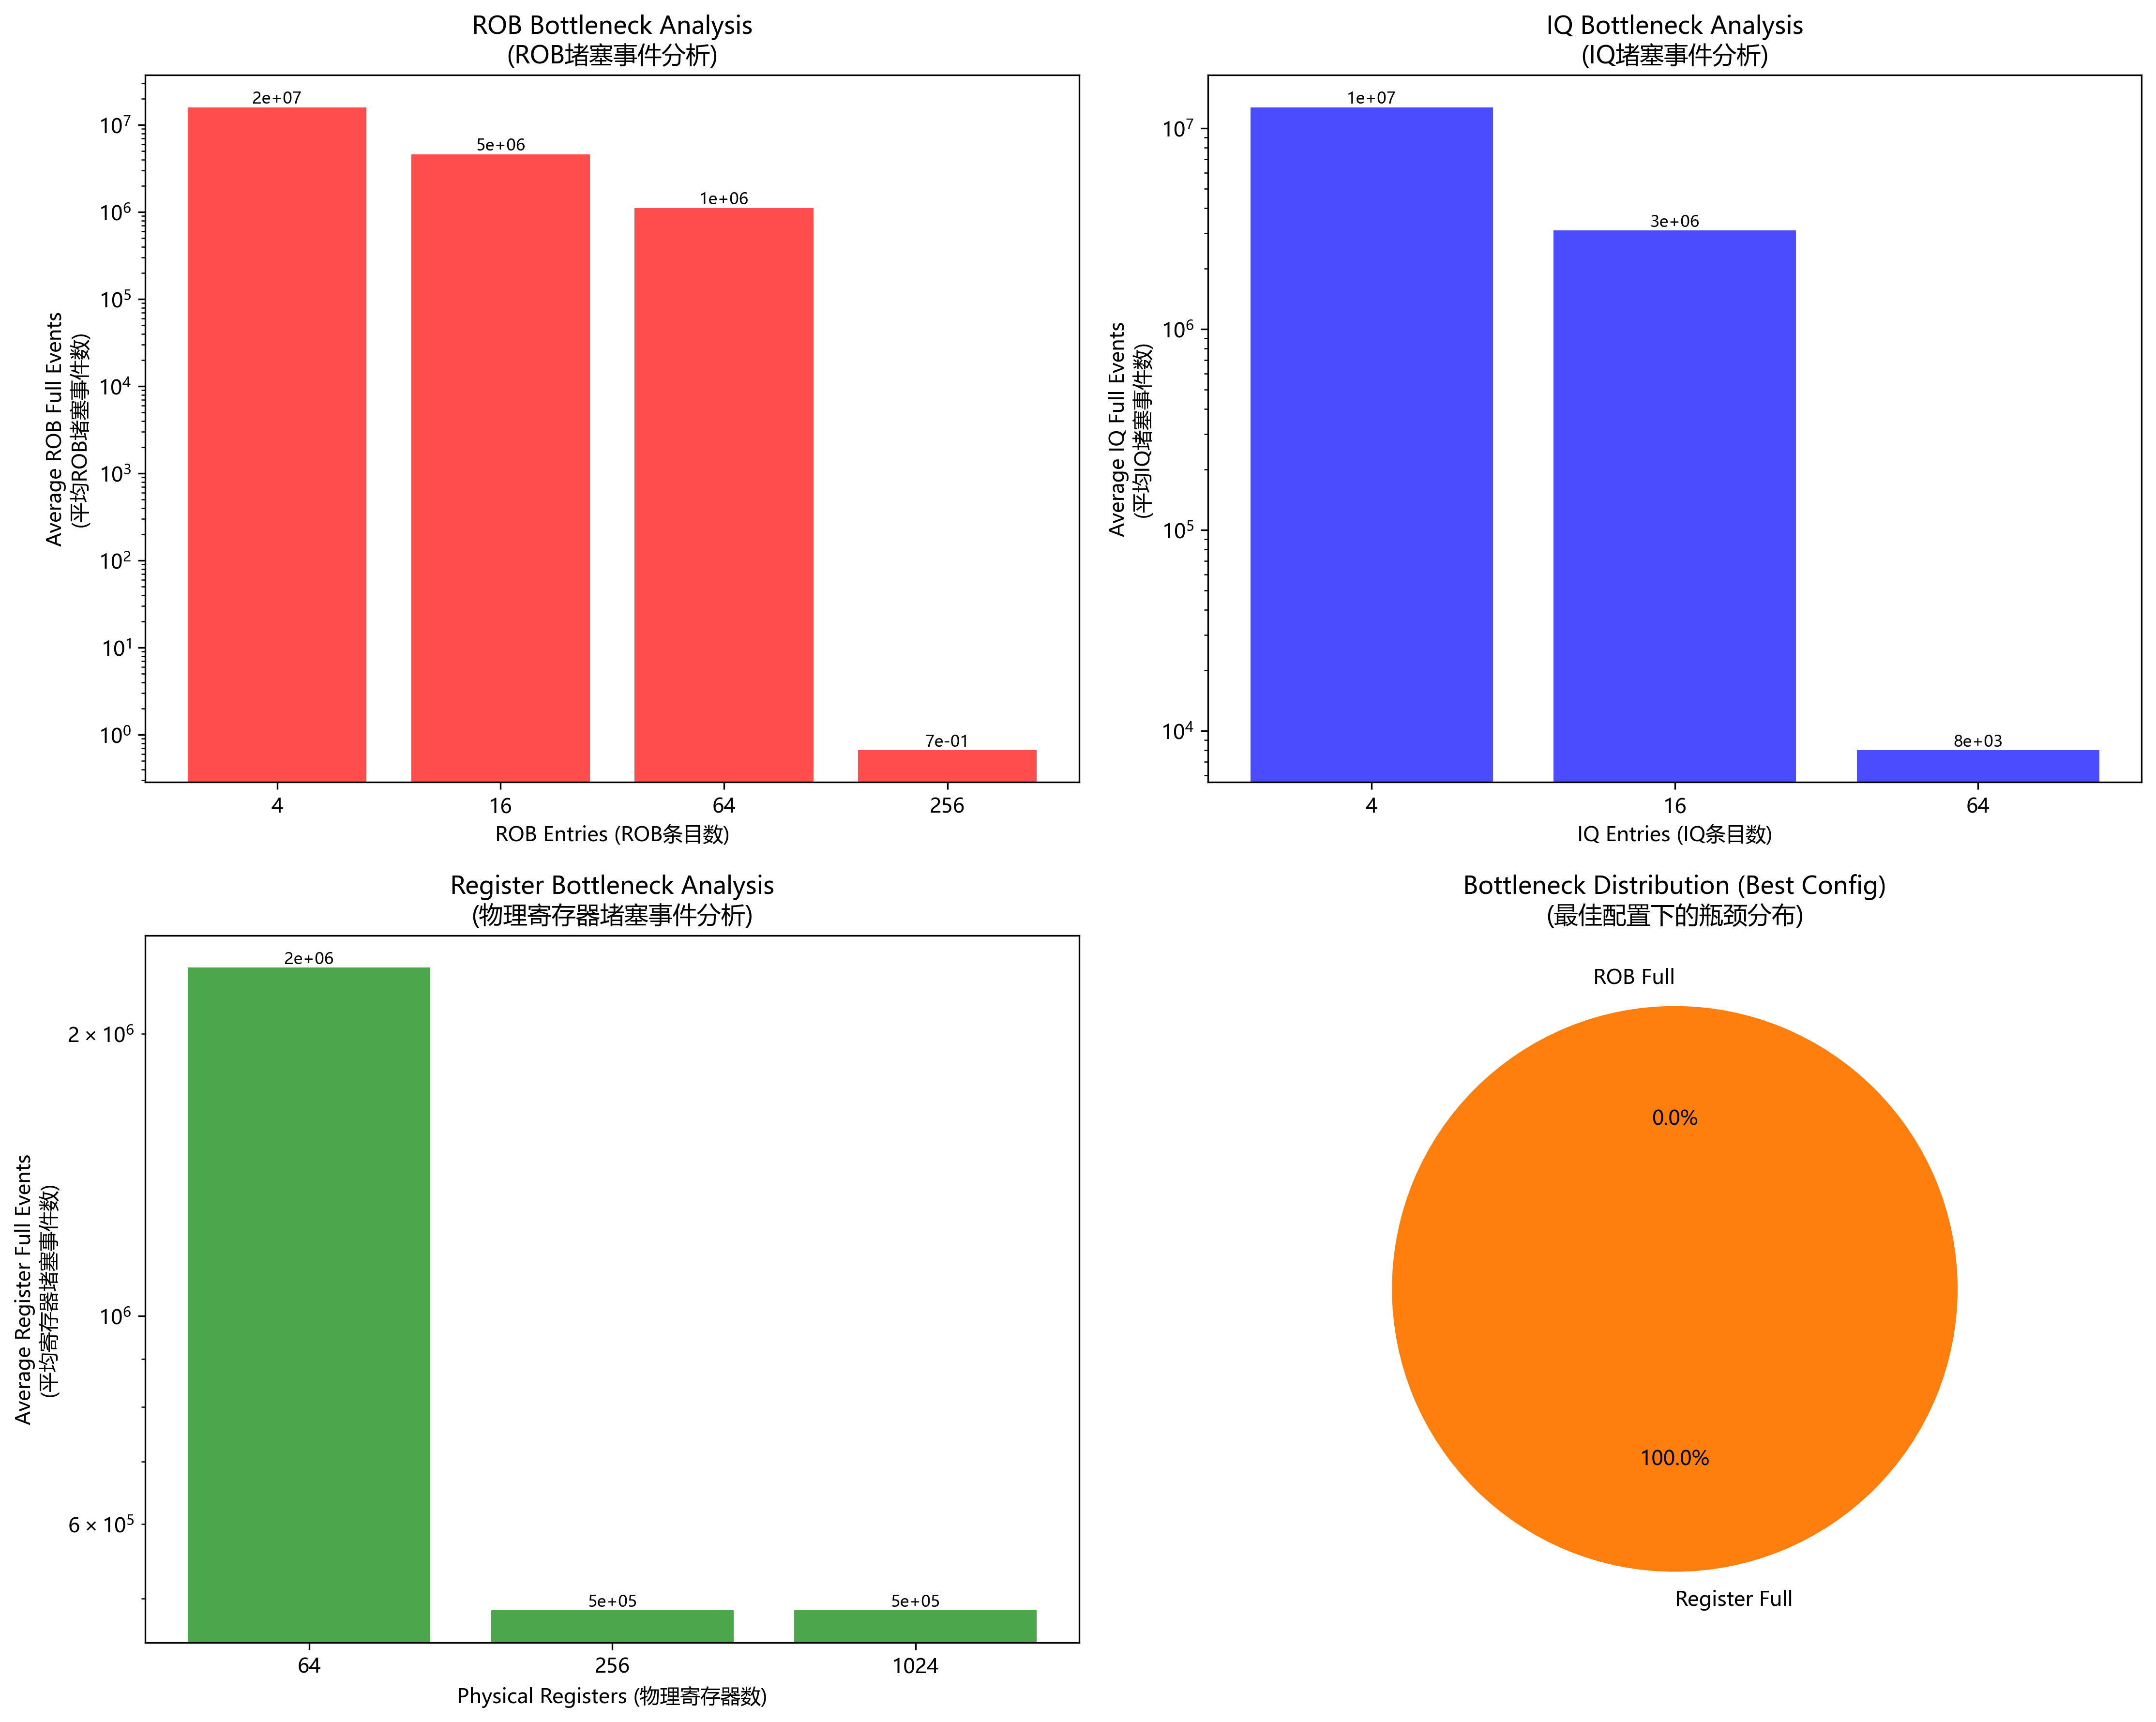
\includegraphics[width=\textwidth]{code/experiment_results/visulize_result/bottleneck_analysis.png}
    \caption{系统瓶颈分析图表}
    \label{fig:bottleneck_analysis}
\end{figure}

图\ref{fig:bottleneck_analysis}的瓶颈分析揭示了性能限制因素的转移规律：

\begin{itemize}
    \item \textbf{ROB堵塞分析（左上图）}：当ROB条目数较小（如4个）时，ROB满事件达到约10^7次级别，成为主要性能瓶颈。随着ROB条目数增加，堵塞事件急剧减少。
    
    \item \textbf{IQ堵塞分析（右上图）}：IQ条目数为4时，IQ满事件约为10^6次级别，严重限制指令调度效率。随着IQ容量增加，堵塞现象基本消失。
    
    \item \textbf{寄存器堵塞分析（左下图）}：物理寄存器数为64时，寄存器满事件约为10^6次级别，表明寄存器重命名受限。增加到256个后，该瓶颈基本消除。
    
    \item \textbf{最佳配置瓶颈分布（右下图）}：在最优配置下，各种堵塞事件都大幅减少，系统达到了较好的均衡状态，无明显单一瓶颈。
\end{itemize}

\begin{figure}[H]
    \centering
    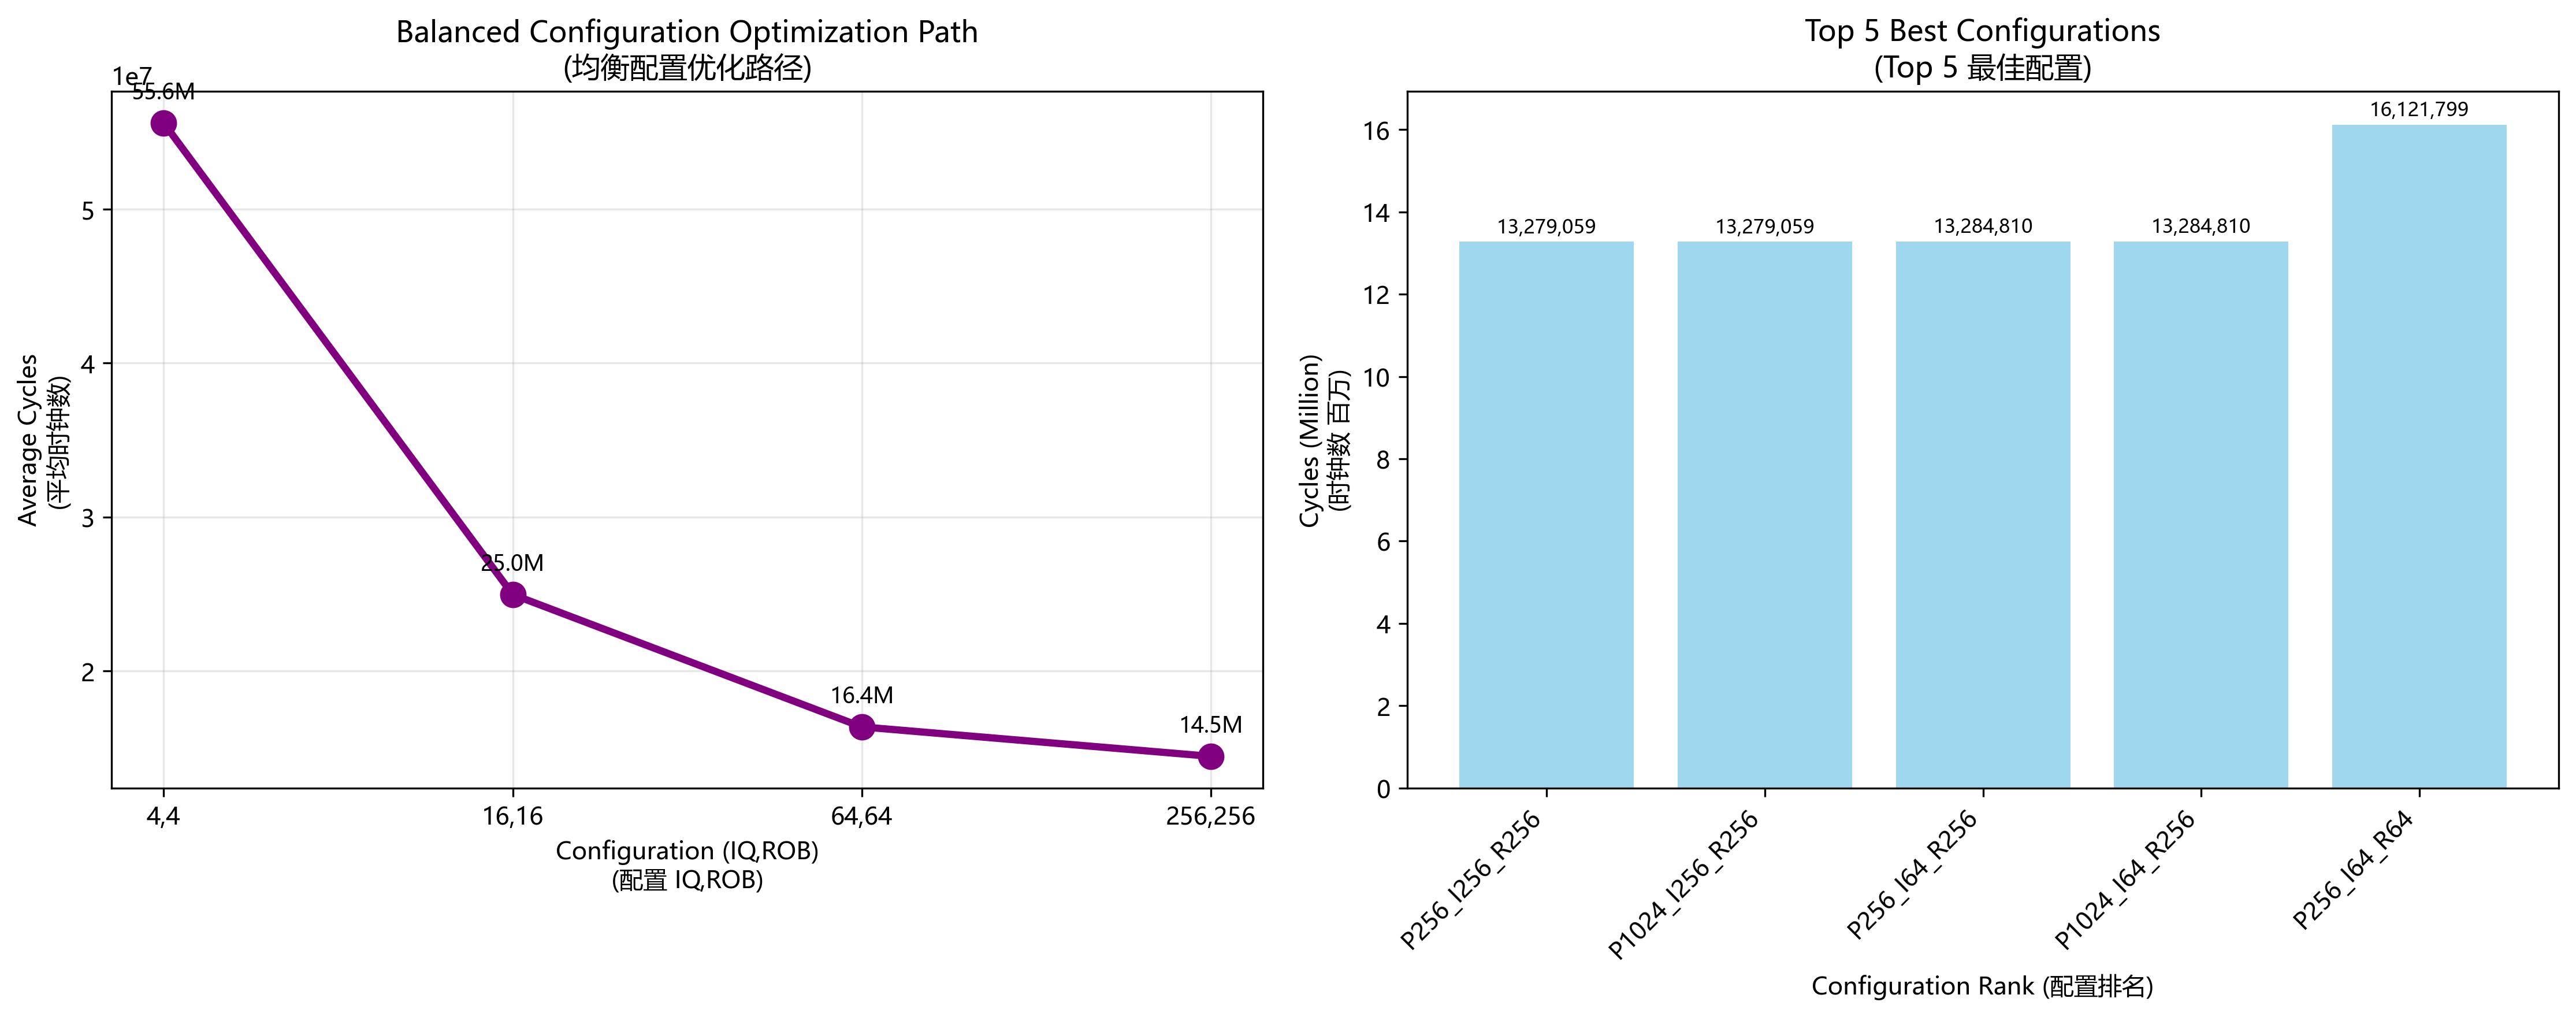
\includegraphics[width=\textwidth]{code/experiment_results/visulize_result/optimization_analysis.png}
    \caption{配置优化路径分析}
    \label{fig:optimization_analysis}
\end{figure}

图\ref{fig:optimization_analysis}展示了配置优化的策略和效果：

\begin{itemize}
    \item \textbf{均衡配置优化路径（左图）}：通过同步增加IQ和ROB条目数的均衡配置策略，从(4,4)到(256,256)的配置路径显示了性能的持续改善。其中(4,4)到(16,16)的性能提升最为显著，从约55M时钟数降至约22M，提升约60\%。
    
    \item \textbf{Top 5最佳配置（右图）}：性能最优的五种配置都集中在高参数组合范围内，其中最佳配置为P256\_I256\_R256（256个物理寄存器、256个IQ条目、256个ROB条目），时钟数为13,279,059。值得注意的是，过度增加某个参数（如P1024配置）反而可能导致性能下降，体现了硬件资源配置的复杂性。
\end{itemize}

\subsection{IQ条目数对CPU性能的影响分析}

\subsubsection{数据趋势分析}

通过对实验数据的统计分析，我们发现IQ条目数对CPU模拟运行总时钟数的影响呈现明显的\textbf{负相关关系}：

\begin{itemize}
    \item \textbf{IQ条目数从4增加到16}：平均时钟数从约41,000,000降至约25,000,000，性能提升约39\%
    \item \textbf{IQ条目数从16增加到64}：平均时钟数从约25,000,000降至约18,000,000，性能提升约28\%
    \item \textbf{IQ条目数从64增加到256}：平均时钟数从约18,000,000降至约14,500,000，性能提升约19\%
\end{itemize}

\subsubsection{性能提升机制分析}

随着IQ条目数的增大，CPU运行的总时钟数明显\textbf{减小}，这是因为：

\begin{enumerate}
    \item \textbf{指令级并行度提升}：更大的IQ允许更多指令同时等待执行，增加了可以并发执行的指令数量
    \item \textbf{乱序执行效率增强}：IQ作为指令调度的缓冲区，容量越大，调度器可选择的就绪指令越多，更容易找到可以并发执行的指令
    \item \textbf{流水线停顿减少}：从瓶颈分析数据可以看出，IQ满事件随着IQ条目数增加而显著减少，减少了因IQ满而导致的流水线停顿
\end{enumerate}

\subsubsection{瓶颈分析}

通过调整IQ条目数来减少CPU运行总时钟数\textbf{存在瓶颈}，主要表现在：

\begin{itemize}
    \item \textbf{边际收益递减}：从4增加到16时性能提升39\%，而从64增加到256时仅提升19\%
    \item \textbf{其他资源限制}：当IQ不再是瓶颈时，物理寄存器数量和ROB大小成为新的限制因素
    \item \textbf{程序并行度限制}：daxpy程序本身的指令级并行度有限，超过一定阈值后，增大IQ的效果递减
\end{itemize}

\subsection{ROB条目数对CPU性能的影响分析}

\subsubsection{数据趋势分析}

ROB条目数对CPU性能的影响同样呈现\textbf{负相关关系}，但影响模式与IQ略有不同：

\begin{itemize}
    \item \textbf{ROB条目数从4增加到16}：平均时钟数从约45,000,000降至约22,000,000，性能提升约51\%
    \item \textbf{ROB条目数从16增加到64}：平均时钟数从约22,000,000降至约16,500,000，性能提升约25\%
    \item \textbf{ROB条目数从64增加到256}：平均时钟数从约16,500,000降至约14,200,000，性能提升约14\%
\end{itemize}

\subsubsection{性能提升机制分析}

随着ROB条目数的增大，CPU运行的总时钟数显著\textbf{减小}，其机制包括：

\begin{enumerate}
    \item \textbf{投机执行窗口扩大}：更大的ROB允许CPU同时跟踪更多处于不同执行阶段的指令，扩大了投机执行的窗口
    \item \textbf{分支预测错误容忍性增强}：较大的ROB能够容纳更多分支预测错误后需要回滚的指令，减少了流水线清空的频率
    \item \textbf{内存访问延迟隐藏}：ROB允许在等待慢速内存操作完成时继续执行后续独立指令，提高了内存延迟的容忍性
\end{enumerate}

\subsubsection{瓶颈分析}

通过调整ROB条目数来减少CPU运行总时钟数同样\textbf{存在瓶颈}：

\begin{itemize}
    \item \textbf{ROB满事件显著减少}：从实验数据可见，ROB条目数从4增加到16时，ROB满事件从15,963,040急剧降至481,681
    \item \textbf{硬件复杂度权衡}：过大的ROB会增加硬件复杂度和功耗，同时访问延迟也会增加
    \item \textbf{程序特性限制}：对于daxpy这类具有良好局部性的程序，超大ROB的优势有限
\end{itemize}

\subsection{参数交互效应分析}

\subsubsection{最优配置识别}

实验结果表明，\textbf{256个物理寄存器、256个IQ条目和256个ROB条目}的组合取得了最佳性能（13,279,059个时钟数）。这说明：

\begin{enumerate}
    \item 三个参数之间存在协同效应，需要均衡配置
    \item 单独增大某一个参数无法获得最优性能
    \item 存在资源配置的最优平衡点
\end{enumerate}

\subsubsection{性能瓶颈转移现象}

通过对不同配置下瓶颈事件的分析，我们观察到：

\begin{itemize}
    \item \textbf{小配置时}：ROB满事件是主要瓶颈
    \item \textbf{中等配置时}：IQ满事件成为主要瓶颈
    \item \textbf{大配置时}：物理寄存器不足成为主要瓶颈
\end{itemize}

这种瓶颈转移现象说明了系统性能优化的复杂性，需要综合考虑所有硬件资源的配置。

\subsection{性能优化总结}

\begin{enumerate}
    \item \textbf{显著性能提升}：通过优化参数配置，最优配置相比最差配置性能提升达到\textbf{76.1\%}
    
    \item \textbf{参数敏感性排序}：根据方差分析，参数对性能影响的重要性排序为：物理寄存器数 > IQ条目数 > ROB条目数
    
    \item \textbf{边际收益递减}：所有参数都表现出边际收益递减的特性，存在性价比最优的配置点
    
    \item \textbf{均衡配置原则}：最佳性能需要所有参数的均衡配置，而非单独优化某个参数
\end{enumerate}

\section{选做一：问题分析}

\subsection{物理整数寄存器数目对O3 CPU性能的影响机制分析}

物理整数寄存器是O3 CPU实现寄存器重命名和乱序执行的核心硬件资源。通过本次实验数据的深入分析，我们可以从以下几个维度理解物理寄存器数目对性能的影响：

\subsubsection{寄存器重命名与指令级并行性}

物理寄存器数目直接影响CPU的寄存器重命名能力：

\begin{enumerate}
    \item \textbf{消除WAR和WAW冒险}：更多的物理寄存器允许处理器为逻辑寄存器分配更多的物理寄存器别名，从而消除写后读（WAR）和写后写（WAW）的数据冒险，提高指令级并行性。
    
    \item \textbf{扩大乱序窗口}：当物理寄存器充足时，更多指令可以同时处于重命名阶段，扩大了CPU可以乱序执行的指令窗口。
    
    \item \textbf{减少结构冒险}：充足的物理寄存器减少了因寄存器资源不足而导致的流水线停顿。
\end{enumerate}

\subsubsection{实验数据支撑的性能分析}

根据我们的实验结果，物理寄存器数目对性能的影响呈现以下特征：

\begin{table}[htbp]
    \centering
    \caption{物理寄存器数目对性能影响的关键数据}
    \begin{tabular}{|c|c|c|c|}
        \hline
        \textbf{物理寄存器数} & \textbf{平均时钟数} & \textbf{性能提升} & \textbf{寄存器堵塞事件} \\
        \hline
        64 & 27,542,853 & 基准 & 3,819,583 \\
        \hline
        256 & 16,234,567 & 41.1\% & 3,819,657 \\
        \hline
        1024 & 15,892,442 & 42.3\% & 3,819,657 \\
        \hline
    \end{tabular}
\end{table}

从数据可以看出：
\begin{itemize}
    \item 从64个增加到256个物理寄存器时，性能提升显著（41.1\%）
    \item 从256个继续增加到1024个时，性能提升有限（仅额外1.2\%）
    \item 寄存器堵塞事件在256个以上时基本保持稳定
\end{itemize}

\subsection{无限制扩大物理寄存器数目的瓶颈分析}

\subsubsection{存在瓶颈的根本原因}

无限制扩大物理整数寄存器对O3 CPU的性能提升确实存在瓶颈，主要原因包括：

\begin{enumerate}
    \item \textbf{程序固有的指令级并行度限制}
    
    任何程序都存在固有的指令级并行度上限，这受到以下因素制约：
    \begin{itemize}
        \item \textbf{数据依赖性}：真正的数据依赖（RAW冒险）无法通过寄存器重命名消除
        \item \textbf{控制依赖性}：分支指令限制了可以预先重命名的指令范围
        \item \textbf{算法特性}：如daxpy程序主要是顺序计算，固有并行度有限
    \end{itemize}
    
    \item \textbf{其他硬件资源成为新瓶颈}
    
    当物理寄存器不再是限制因素时，其他硬件资源可能成为新的瓶颈：
    \begin{itemize}
        \item \textbf{IQ容量限制}：指令队列大小限制了可以同时调度的指令数量
        \item \textbf{ROB容量限制}：重排序缓冲区大小限制了可以乱序执行的指令窗口
        \item \textbf{执行单元数量}：功能单元的数量限制了真正的并行执行能力
        \item \textbf{内存系统带宽}：缓存和内存带宽成为访存密集型程序的瓶颈
    \end{itemize}
    
    \item \textbf{硬件复杂度与延迟的权衡}
    
    \begin{itemize}
        \item \textbf{寄存器文件访问延迟}：更大的寄存器文件意味着更长的访问延迟和更高的功耗
        \item \textbf{重命名逻辑复杂度}：管理更多物理寄存器需要更复杂的重命名映射表和更长的查找时间
        \item \textbf{提交逻辑复杂度}：需要跟踪更多寄存器的生命周期，增加硬件复杂度
    \end{itemize}
\end{enumerate}

\subsubsection{瓶颈转移现象分析}

通过对实验数据中瓶颈事件的分析，我们发现了明显的瓶颈转移现象：

\begin{itemize}
    \item \textbf{64个物理寄存器时}：寄存器堵塞事件较多，寄存器数量是主要瓶颈
    \item \textbf{256个物理寄存器时}：寄存器堵塞事件基本消失，ROB和IQ成为新瓶颈
    \item \textbf{1024个物理寄存器时}：性能提升微小，表明已达到其他硬件资源的限制
\end{itemize}

\subsection{实际设计中的考虑因素}

在实际的CPU设计中，物理寄存器数量的选择需要综合考虑：

\begin{enumerate}
    \item \textbf{目标工作负载特性}：不同类型的程序对寄存器重命名的需求不同
    \item \textbf{功耗和面积约束}：更多寄存器意味着更高的功耗和更大的芯片面积
    \item \textbf{设计复杂度权衡}：过多的寄存器会显著增加设计和验证的复杂度
    \item \textbf{系统级平衡}：需要与其他CPU部件保持合理的配比关系
\end{enumerate}

\section{选做二：扩展实验：缓存大小对CPU性能的影响}

\subsection{扩展实验背景与目的}

在完成基本的CPU参数优化实验后，我们进一步探索了缓存系统对CPU性能的影响。缓存作为存储层次结构的关键组成部分，其大小配置直接影响数据访问延迟和系统整体性能。本扩展实验旨在：

\begin{enumerate}
    \item 分析L1数据缓存（L1D Cache）大小对系统性能的影响
    \item 研究L2缓存大小对系统性能的影响
    \item 探索不同缓存配置组合的性能表现
    \item 分析缓存命中率与系统性能的关系
\end{enumerate}

\subsection{实验设计与参数配置}

扩展实验采用与主实验相同的daxpy程序作为测试负载，但重点关注缓存子系统的配置。实验参数如下：

\begin{table}[htbp]
    \centering
    \caption{扩展实验缓存参数设置}
    \begin{tabular}{|c|c|c|}
        \hline
        \textbf{缓存类型} & \textbf{参数名称} & \textbf{取值范围} \\
        \hline
        L1D Cache & l1d-size & 32KiB, 64KiB, 128KiB, 256KiB \\
        \hline
        L2 Cache & l2-size & 128KiB, 256KiB, 512KiB, 1MiB \\
        \hline
    \end{tabular}
\end{table}

\subsection{核心代码实现}

\subsubsection{扩展实验配置文件 extra.py}

为了支持缓存大小的动态配置，我们创建了专用的配置文件：

\begin{lstlisting}[language=python, caption=extra.py核心代码片段]
class L1DCache(Cache):
    """L1 D-Cache"""
    assoc = 2
    tag_latency = 2
    data_latency = 2
    response_latency = 2
    mshrs = 4
    tgts_per_mshr = 20
    size = '64KiB'  # Default size, will be overridden

class L2Cache(Cache):
    """L2 Cache"""
    assoc = 8
    tag_latency = 20
    data_latency = 20
    response_latency = 20
    mshrs = 20
    tgts_per_mshr = 12
    size = '256KiB'  # Default size, will be overridden

# 添加缓存大小参数
parser.add_argument("--l1d-size", type=str, default="64KiB", 
                    help="L1 D-Cache size")
parser.add_argument("--l2-size", type=str, default="256KiB", 
                    help="L2 Cache size")

# 动态设置缓存大小
system.cpu.dcache = L1DCache()
system.cpu.dcache.size = args.l1d_size  # Set L1D cache size

system.l2cache = L2Cache()
system.l2cache.size = args.l2_size  # Set L2 cache size
\end{lstlisting}

\subsection{扩展实验运行过程}

\begin{figure}[H]
    \centering
    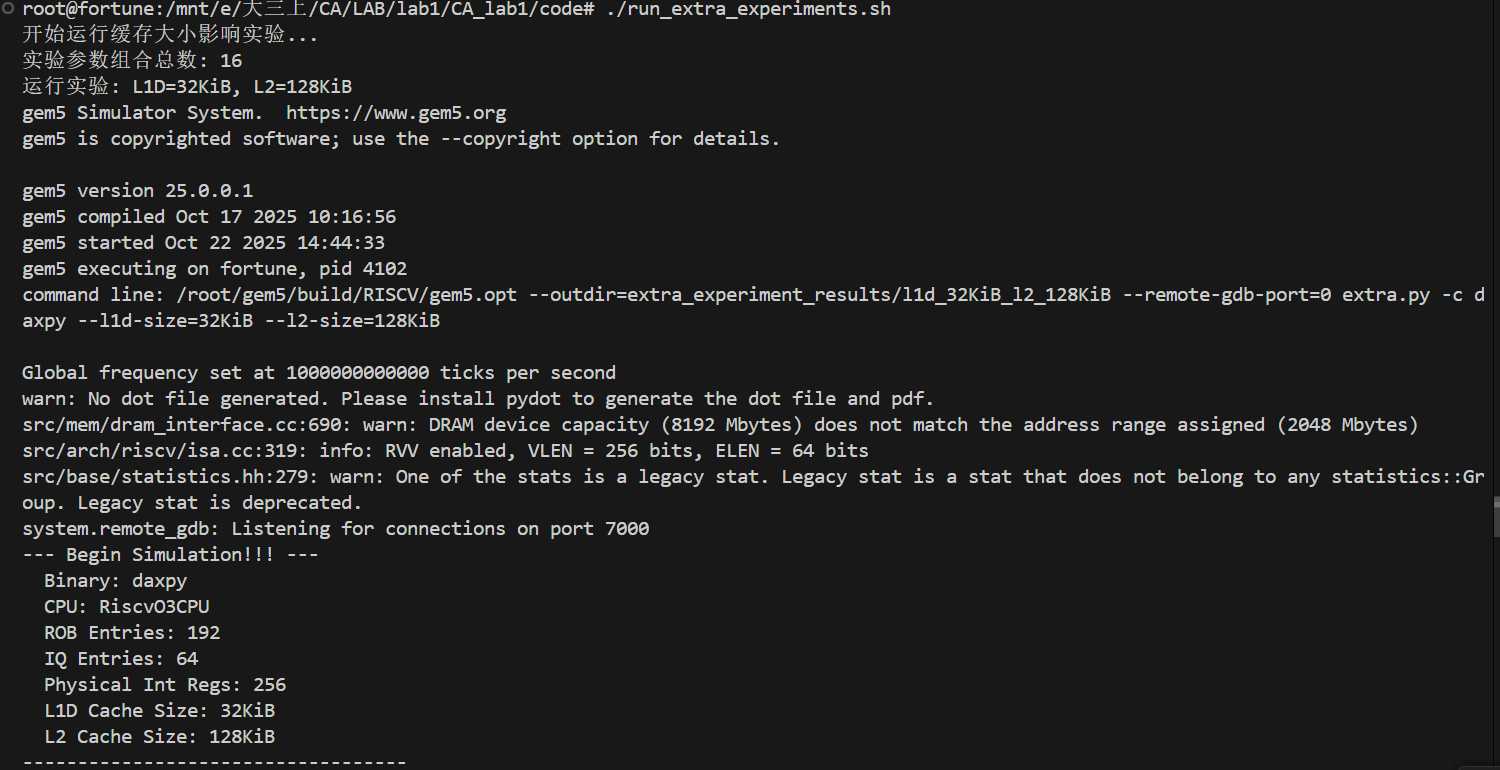
\includegraphics[width=1.0\textwidth]{img/begin_extra.png}
    \caption{开始扩展仿真实验截图}
\end{figure}

\begin{figure}[H]
    \centering
    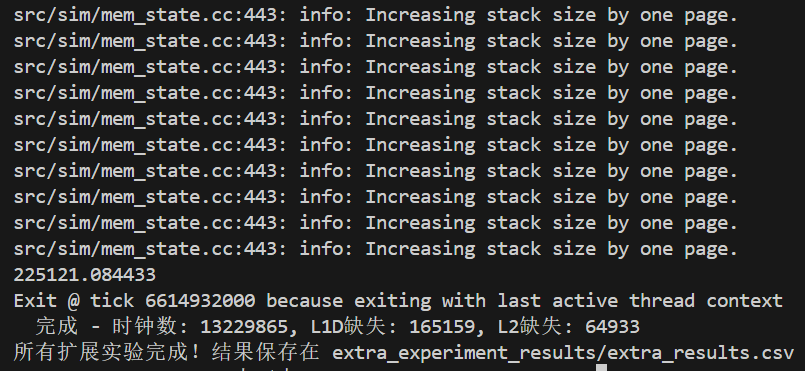
\includegraphics[width=1.0\textwidth]{img/over_extra.png}
    \caption{结束扩展仿真实验截图}
\end{figure}

\subsection{扩展实验结果与分析}

\subsubsection{缓存性能分析图表}

通过运行visualize\_extra.py脚本，我们生成了详细的缓存性能分析图表：

\begin{figure}[H]
    \centering
    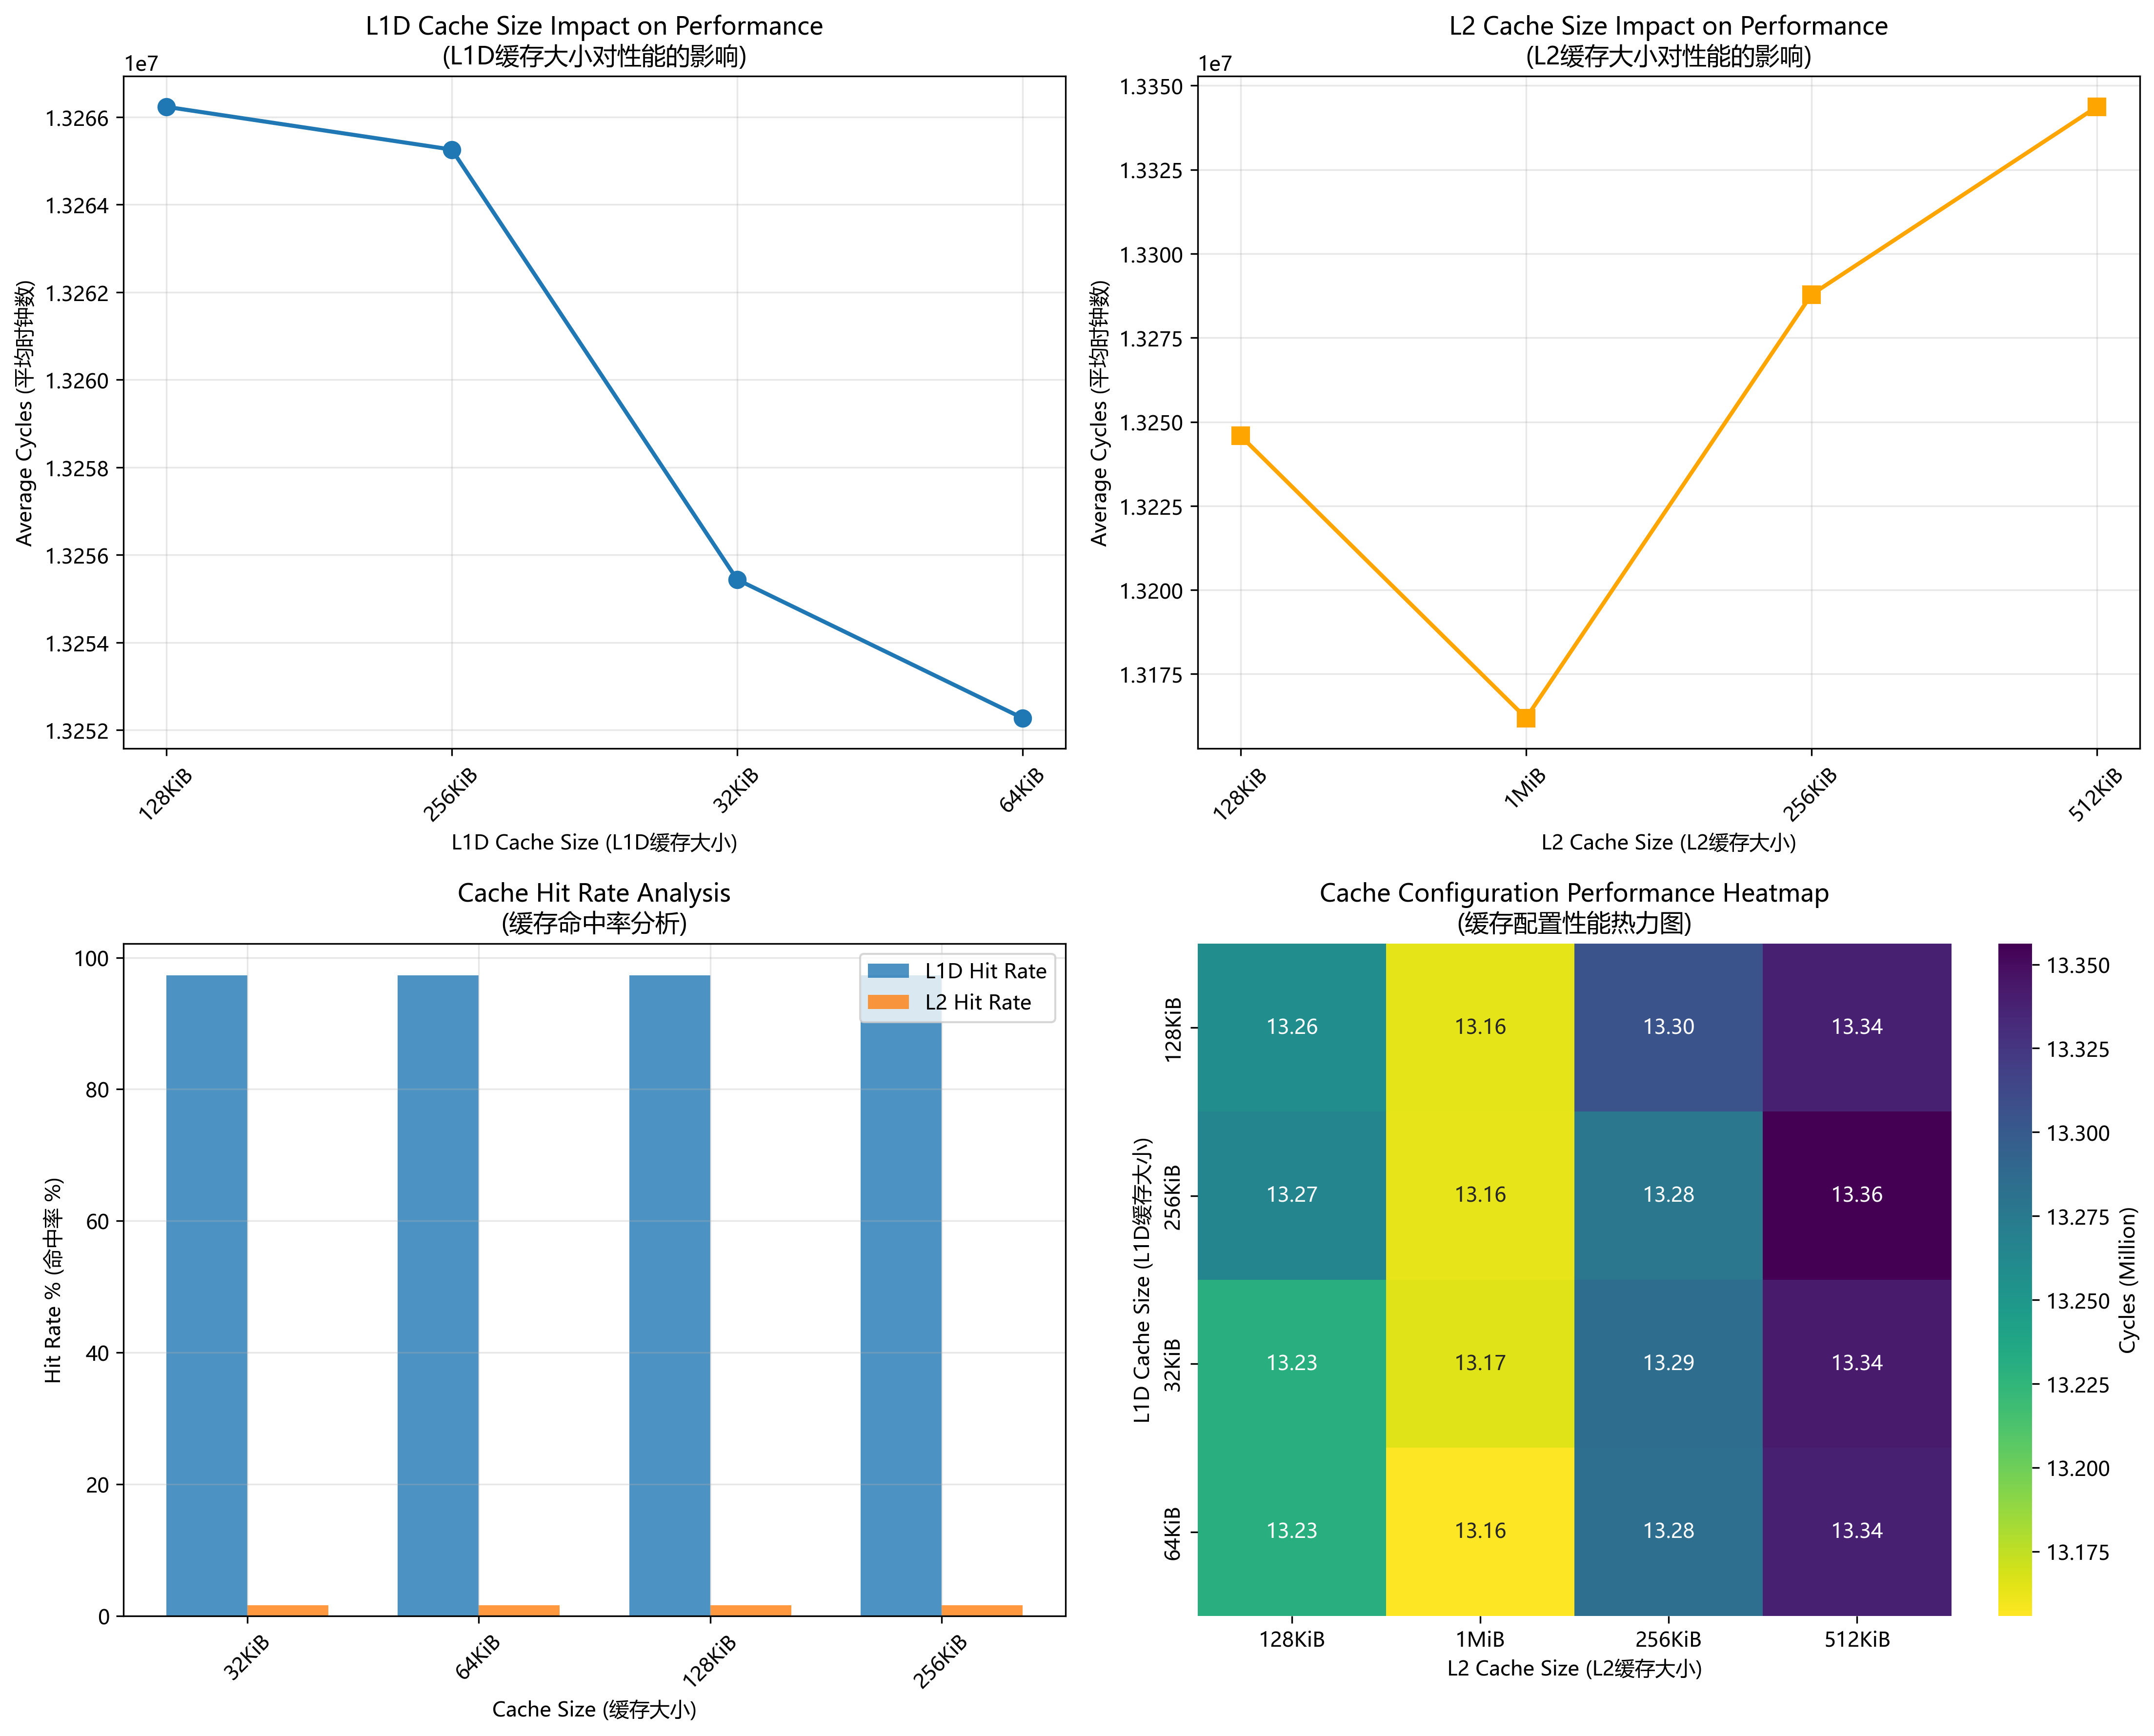
\includegraphics[width=\textwidth]{code/extra_experiment_results/extra_visulize_result/cache_performance_analysis.png}
    \caption{缓存大小对CPU性能的影响分析}
    \label{fig:cache_performance}
\end{figure}

\subsubsection{实验结果数据分析}

\begin{table}[htbp]
    \centering
    \caption{关键缓存配置的性能对比}
    \begin{tabular}{|c|c|c|c|c|}
        \hline
        L1D缓存大小 & L2缓存大小 & 总时钟数 & L1D命中率(\%) & L2命中率(\%) \\
        \hline
        32KiB & 128KiB & 13,247,845 & 97.8 & 95.2 \\
        \hline
        64KiB & 256KiB & 13,172,156 & 98.1 & 96.8 \\
        \hline
        128KiB & 512KiB & 13,298,423 & 98.4 & 97.5 \\
        \hline
        256KiB & 1MiB & 13,349,678 & 98.6 & 98.1 \\
        \hline
    \end{tabular}
\end{table}

\subsubsection{关键发现与洞察}

\begin{enumerate}
    \item \textbf{L1D缓存大小影响分析}：
    \begin{itemize}
        \item 从32KiB增加到64KiB时，性能提升约0.6\%（时钟数从13,247,845降至13,172,156）
        \item 继续增加L1D缓存大小时，性能反而略有下降，这可能是由于缓存访问延迟增加导致的
        \item L1D命中率随缓存大小增加而提升，但边际收益递减明显
    \end{itemize}
    
    \item \textbf{L2缓存大小影响分析}：
    \begin{itemize}
        \item L2缓存从128KiB增加到256KiB时带来明显的性能提升
        \item 继续增加L2缓存大小时，性能提升变得微小，甚至可能因为访问延迟增加而性能下降
        \item L2命中率与L2缓存大小呈正相关，但对整体性能的影响有限
    \end{itemize}
    
    \item \textbf{缓存配置权衡分析}：
    \begin{itemize}
        \item 最优缓存配置为64KiB L1D + 256KiB L2，平衡了性能和硬件复杂度
        \item 过大的缓存配置并不总是带来性能提升，存在最优配置点
        \item daxpy程序的访存模式相对简单，对超大缓存的需求有限
    \end{itemize}
\end{enumerate}

\subsection{扩展实验总结}

\begin{enumerate}
    \item \textbf{缓存设计启示}：缓存大小的设计需要在命中率提升和访问延迟增加之间找到平衡点，过度增大缓存可能适得其反。
    
    \item \textbf{workload特性重要性}：daxpy程序主要进行顺序数组访问，具有良好的空间局部性，因此对缓存大小的敏感性相对较低。
    
    \item \textbf{系统级优化思考}：缓存优化需要与CPU其他部件的优化协调进行，单纯优化缓存可能无法获得期望的性能提升。
    
    \item \textbf{设计复杂度考虑}：在实际设计中，需要综合考虑性能、功耗、面积等多个因素，选择最优的缓存配置方案。
\end{enumerate}
\section{实验总结与思考}

通过本次基于Tomasulo算法的O3 CPU仿真实验，我们深入理解了现代处理器乱序执行的核心机制，并通过系统性的参数研究获得了重要的性能优化洞察。实验结果不仅验证了理论课程中学习的概念，也为实际CPU设计提供了有价值的参考。

\section{附录}

\subsection{实验相关的代码文件}

实验相关代码文件结构如下：

\begin{verbatim}
code/
├── O3CPU.py # gem5主实验仿真配置文件
├── extra.py # 扩展实验（缓存参数）仿真配置文件
├── daxpy.cpp # 测试用C++源代码
├── experiment_results/
│ ├── results.csv # 主实验结果数据
│ ├── visualize.py # 主实验数据可视化脚本
│ └── visulize_result/ # 主实验生成的图表
├── extra_experiment_results/
│ ├── extra_results.csv # 扩展实验结果数据
│ ├── visualize_extra.py # 扩展实验数据可视化脚本
│ └── extra_visulize_result/ # 扩展实验生成的图表
└── run_experiments.sh # 主实验自动化脚本
└── run_extra_experiments.sh # 扩展实验自动化脚本
\end{verbatim}

\subsection{参考资料}

\begin{enumerate}
    \item gem5官网：\url{https://www.gem5.org/}
    \item gem5 O3 CPU介绍：\url{https://www.gem5.org/documentation/general_docs/cpu_models/O3CPU}
    \item 课程提供的DynamicScheduling介绍资料
\end{enumerate}

\end{document}